\section{Activation functions}

Activation functions play a critical role in neural networks by introducing non-linearity into the model. 
Common activation functions include:
\begin{itemize}
    \item \textit{Linear}: $g(a)=a$ with a derivative of $g^\prime (a)=1$. 
    \item \textit{Sigmoid}: $g(a)=\dfrac{1}{1+e^{-a}}$ with a derivative of $g(a)(1-g(a))$. 
        This function is widely used due to its simplicity and ability to model probabilities.
    \item \textit{Hyperbolic tangent} (Tanh): $g(a)=\frac{e^a-e^{-a}}{e^a+e^{-a}}$ with a derivative of $1-g(a)^2$.
        This function is often preferred for hidden layers as it outputs values in the range $[-1,1]$, centering the data.
\end{itemize}
The choice of the activation function is a design decision, influenced by the nature of the task and the structure of the network.

\subsection{Output layer}
The activation function for the output layer depends on the type of problem being addressed:
\begin{itemize}
    \item \textit{Regression}: in regression tasks, where the output spans the real number domain $\mathbb{R}$, a linear activation function is typically used for the output neuron.
    \item \textit{Binary classification}: the choice of activation depends on the coding of the class labels: 
        \begin{enumerate}
            \item For classes coded as $\Omega_0=-1$, $\Omega_1=1$, a Tanh activation function is appropriate. 
            \item For classes coded as $\Omega_0=0$, $\Omega_1=1$, a Sigmoid activation function is commonly used, as it can be interpreted as representing the posterior probability of a class.
        \end{enumerate}
    \item \textit{Multi-class classification}: for problems with $K$ classes, the output layer contains $K$ neurons, one for each class. 
        The classes are typically encoded using one-hot encoding, e.g., $\Omega_0=\begin{bmatrix} 0 & 0 & 1 \end{bmatrix}$, $\Omega_1=\begin{bmatrix} 0 & 1 & 0 \end{bmatrix}$, and $\Omega_2=\begin{bmatrix} 1 & 0 & 0 \end{bmatrix}$.
        The output neurons utilize a softmax activation function:
        \[y_k=\dfrac{e^{z_k}}{\sum_ke^{z_k}}=\dfrac{e^{\sum_jw_{kj}h_j(\sum_i^Iw_{ji}x_i)}}{\sum_{k=1}^Ke^{\sum_jw_{kj}h_j(\sum_i^Iw_{ji}x_i)}}\]
        Here, $z_k$ is the activation value of the $k$-th output neuron. 
        The softmax function normalizes the output vector, providing class probabilities.
\end{itemize}

\subsection{Hidden layers}
For the hidden layers, activation functions such as the Sigmoid or Tanh are commonly used. 
These functions introduce non-linearity, allowing the network to model complex patterns in the data.
\begin{theorem}
    A single hidden layer feedforward neural network with S-shaped activation functions (such as Sigmoid or Tanh) can approximate any measurable function to any desired degree of accuracy on a compact set.
\end{theorem}
This theorem implies that a single hidden layer can theoretically represent any function, though it does not guarantee that the learning algorithm will find the necessary weights. 
In practice, an excessively large number of hidden units may be required, and the network may struggle to generalize, particularly if overfitting occurs. 
However, for classification tasks, typically only one additional hidden layer is needed to achieve satisfactory performance.

\subsection{Alternative activation functions}
Activation functions like sigmoid or hyperbolic tangent tend to saturate, meaning their gradients become close to zero, or at least less than one, in many cases. 
Since backpropagation relies on gradient multiplication, this saturation causes gradients to vanish as they propagate backward through the network. 
This leads to the well-known vanishing gradient problem, where learning becomes extremely slow or even impossible, especially in deep networks. 
Although this problem is particularly evident in Recurrent Neural Networks, it also affects deep feed-forward networks, and for a long time, it was a significant obstacle to neural network training.

A popular solution to this issue is the Rectified Linear Unit (ReLU) activation function, defined as:
\[g(a)=\text{ReLU}(a=\max(0,a))\]
Its derivative is:
\[g^\prime(a)=1_{a>0}\]
ReLU has several notable advantages:
\begin{itemize}
    \item \textit{Faster convergence}: stochastic Gradient Descent converges approximately six times faster with ReLU compared to sigmoid or tanh activations.
    \item \textit{Sparse activation}: since only a portion of the hidden units are activated (i.e., those with positive input), this leads to a more efficient representation.
    \item \textit{Efficient gradient propagation}: ReLU avoids both the vanishing and exploding gradient problems, making it easier to train deep networks.
    \item \textit{Efficient computation}: ReLU is computationally efficient, as it only involves simple thresholding at zero.
    \item \textit{Scale-invariance}: the output of ReLU is invariant to the scale of its input, meaning $\max(0,xa)=a\max(0,x)$.
\end{itemize}
\begin{figure}[H]
    \centering
    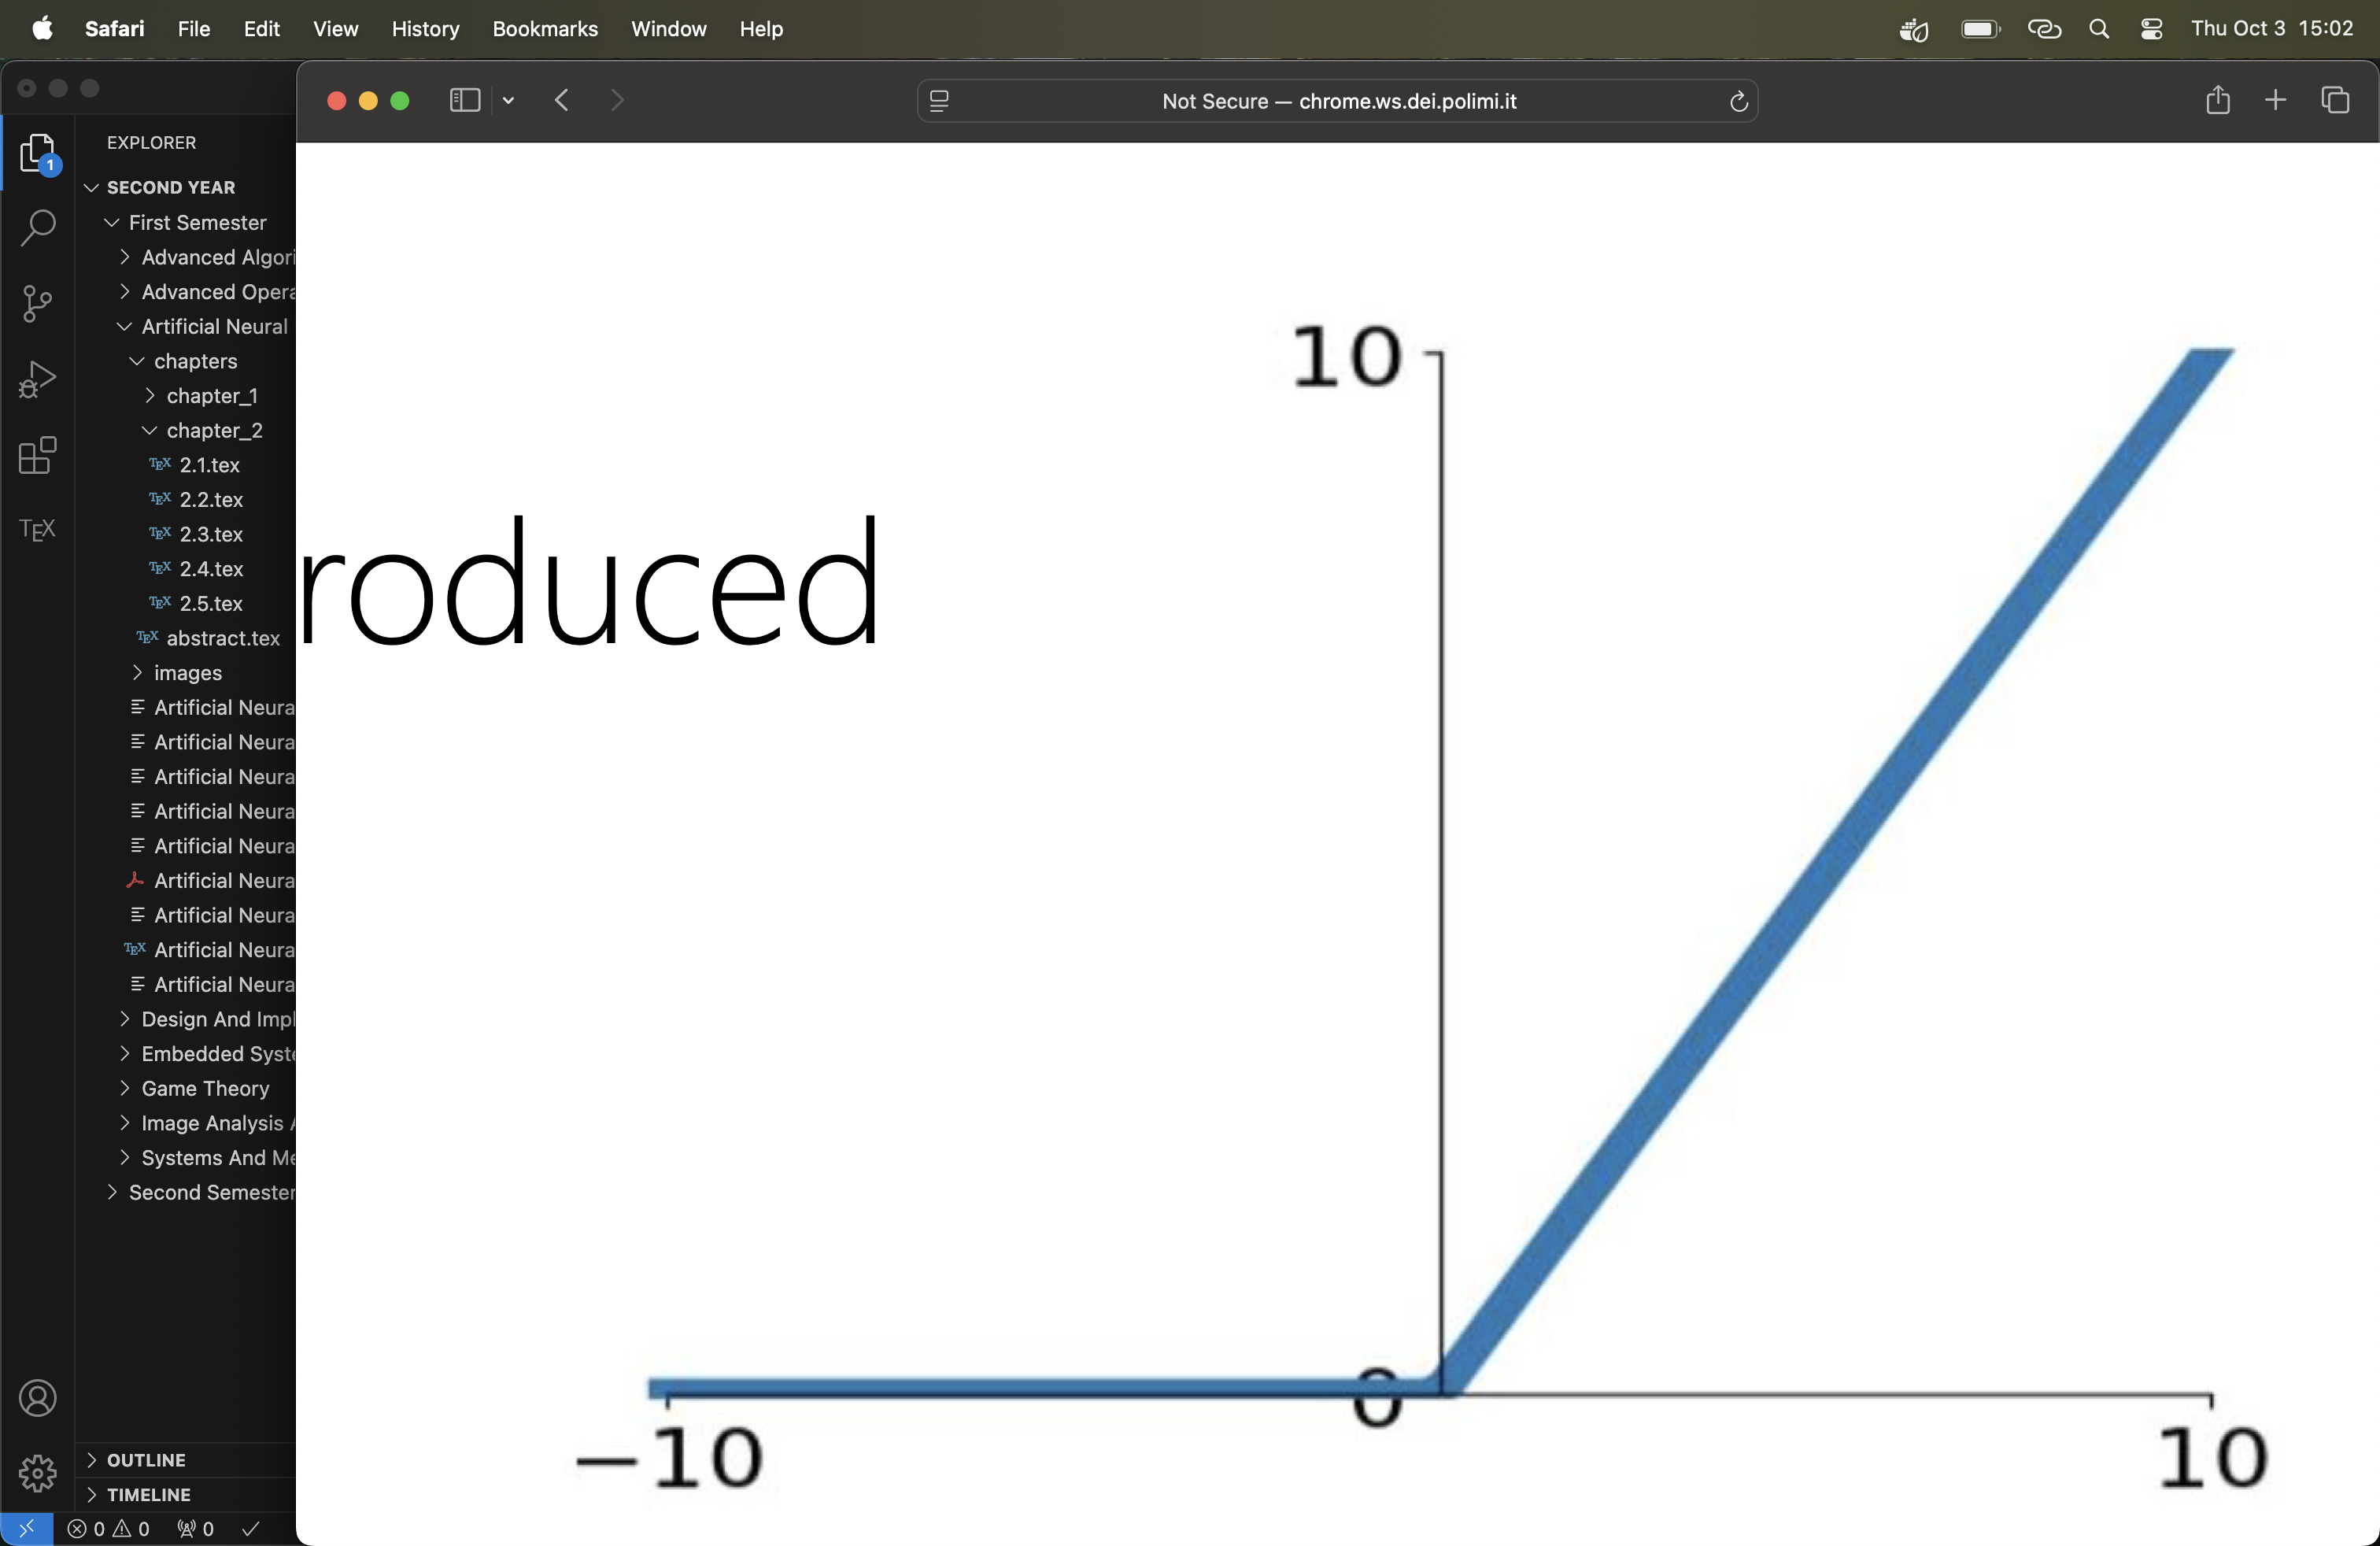
\includegraphics[width=0.5\linewidth]{images/relu.png}
    \caption{Rectified Linear Unit}
\end{figure}
Despite its advantages, ReLU has some potential downsides:
\begin{itemize}
    \item \textit{Non-differentiability at zero}: while ReLU is non-differentiable at zero, it is differentiable everywhere else. 
        This non-differentiability rarely causes significant issues in practice.
    \item \textit{Non-zero centered output}: ReLU outputs are non-zero-centered, which can lead to imbalanced updates when using gradient descent.
    \item \textit{Unbounded output}: since ReLU does not cap its output, the activations can grow very large, potentially leading to exploding gradients under high learning rates.
    \item \textit{Dying neurons}: a key issue with ReLU is the dying neuron problem, where neurons can get stuck with negative outputs for all inputs. 
        When this happens, their gradients become zero, effectively killing those neurons, as they stop updating during training.
\end{itemize}

\paragraph*{ReLU variants}
Several variants of ReLU have been developed to address some of its limitations:
\begin{itemize}
    \item \textit{Leaky ReLU}: this variant addresses the dying ReLU problem by allowing a small, non-zero gradient for negative input values:
        \[f(x)=\begin{cases}
            x \qquad\qquad \text{if } x \geq 0 \\
            0.01x \qquad\: \text{otherwise}
        \end{cases}\]
        By using a small slope for negative inputs, Leaky ReLU ensures that neurons are less likely to die.
    \item \textit{Exponential Linear Unit} (ELU): ELU aims to bring mean activations closer to zero, which can accelerate learning. 
        It introduces an alpha parameter that controls the saturation for negative values:
        \[f(x)=\begin{cases}
            x \qquad\qquad\quad\:\: \text{if } x \geq 0 \\
            \alpha(e^x-1) \qquad \text{otherwise}
        \end{cases}\]
        The $\alpha$ parameter is typically tuned by hand, and ELU provides smoother, more balanced outputs.
\end{itemize}
